\documentclass[10pt]{article}
\usepackage[english]{babel}
\usepackage[utf8]{inputenc}
\usepackage[OT1]{fontenc}
\usepackage{amsfonts, amsmath, amsthm, amssymb}
\usepackage{graphicx}
\usepackage{listings}
\usepackage[margin=1in]{geometry}
\usepackage{brad}




\title{Using the Gauss-Bonnet Theorem}
\author{Bradley McCoy}
\date{\today}
\begin{document}
\maketitle \tableofcontents 

\section{Preface}

Using the borsuk-ulam theorem rules \cite{jm08}.
Several applications are given in do Carmo \cite{doc76}.
We highlight a subset of these.











\section{Manifolds, Curvature, and the Euler Characteristic}
\label{sec:cast}


The Gauss-Bonnet theorem is a bridge. On one shore is topology and
on the opposite shore geometry. This bridge can be traveled in both directions.
That is, if one has geometric information one can deduce topological information and
if one has topological information one can deduce geometric information.
In symbols, the theorem can be stated as follows

\begin{equation} \label{eqn:g-b}
\int_M K dA + \int_{\partial M} k_g ds = 2\pi \chi(M).
\end{equation}
In this section, we define these symbols.

\subsection{Preliminaries}

We begin with some definitions a that may already be familiar to the reader,
\begin{definition}[Topological Space \cite{munkres}]
A \EMPH{topology} is a pair $(X,\tau)$, where $X$ is a set and
 $\tau$ is a collection of subsets $X$
satisfying:
	\begin{itemize}
		\item $\emptyset$ and $X$ are in $\tau.$
		\item the union of \emph{any} subcollection of elements in $\tau$ is  in $\tau.$
		\item the intersection of any \emph{finite} subcollection of elements in the $\tau$ is in $\tau.$
	\end{itemize}
A set $X$ with a specified topology $\tau$ is called a \EMPH{topological space}.
\end{definition}

We will work with a special type of topological spaces called manfiolds.

\begin{definition}[Manifold  \cite{tu2011}]
	A topological space $M$ is \EMPH{locally Euclidean of dimension $n$}
	if every point $p$ in $M$has a neighborhood $U$ such that there is  a
	homeomorphism  $\phi$ from $U$ into and open  subset of $\R^n$.
	We call the pair $(U,\phi: U\to \R^n)$ a \EMPH{chart}, $U$ a \EMPH{coordinate neighborhood}
	and  $\phi$ a \EMPH{coordinate map}. 
A \EMPH{manifold} is a Hausdorff, second countable, locally Euclidean space.
\end{definition}

The symbol $M$ in \eqnref{g-b} is a manifold. For the most part, we will consider two dimensional manifolds that are called \emph{surfaces}.
We will consider both continuous and discrete objects.
For computational purposes, we often want a combinatorial structure on our manifolds.
This structure will often come in the form a triangulation, which we now define.


\begin{definition}[Independent Points]
Let $v_0,v_1,\ldots,v_k$ be points in $\R^n$. We call them \EMPH{affinely dependent}
if there are real numbers $\alpha_0,\alpha_1,\ldots,\alpha_k$, not all 0, such that
$\Sigma_{i=0}^k \alpha_iv_i=0$ and $\Sigma_{i=0}^k \alpha_i=0.$
Otherwise,  $v_0,v_1,\ldots,v_k$ are \EMPH{affinely independent}.

\end{definition}

\begin{definition}[Simplices]
A \EMPH{simplex} $\sigma$ is the convex hull of a finite affinely independent
set $A$ in $\R^n$. The points in  $A$ are  called vertices, the dimension
of  $\sigma$ is $|A|-1$.  The convex hull of a subset of vertices of a simplex
$\sigma$ is a \EMPH{face} of $\sigma$.
\end{definition}

\begin{definition}[Simplicial Complex]
A nonempty family $C$ of simplices is a \EMPH{simplicial complex} if the following
are satisfied:
\begin{itemize}
\item  Each face of any simplex is a simplex.
\item The intersection of $\sigma_1 \cap \sigma_2$ is a face of both $\sigma_1$ and 
$\sigma_2$.
\end{itemize}


\end{definition}

For many of our applications we will consider a special type of manifold called
a triangular mesh. Meshes are used extensively in graphics.


\begin{definition}[Homeomorphism]
A  \EMPH{homeomorphism}  of topological spaces $(X_1,\tau_1$ and $(X_2,\tau_2)$
is a bijection $\phi:X_1\to X_2$ such that for every $\phi$ and $\phi^{-1}$ are continuous.
\end{definition}
For two topological spaces $X$ and $Y$ if there exists a  homeomorphism between
$X$ and $Y$ we say $X$ and $Y$ are topologically  equivalent and write  $X\cong Y.$

\begin{definition}[Triangulation]
For a topological space $X$ and simplicial complex $C$ if $X\cong C$,
then $C$  is a \EMPH{triangulation} of $X$.
\end{definition}

Often, it is useful to approximate smooth surfaces with fine triangulations called
a \emph{mesh}. We will see meshes in many of our applications.

\subsection{Curvature}

Continuous:

For a curve in $\R^3$ how can we quantify the curvature at a point on the curve?
Let $\gamma$ denote a curve in $\R^3$ and let $p$ be a point on $\gamma$.
We traverse $\gamma$ at unit speed, $\gamma(t)=(x(t),y(t),z(t))$.  
Let $\vec{T}$ denote the unit tangent vector of $\gamma$ at $p$. 
The curvature is how much the tangent vector $\vec{T}=(x'(t),y'(t),z'(t))$ is rotating. 
This is exactly the second derivative $\gamma''$. Since we traverse $\gamma$
at unit speed, $\gamma'(t)^2=1,$ and by the chain rule, $\gamma'\cdot \gamma''=0,$
so  the second derivative is orthogonal to $\gamma'$. The norm of the second
derivative is the curvature $k$.
Let $n$ denote a unit vector parallel to $\gamma''$, then $\gamma''=k n$.
By taking the cross product of $N$ and $T$ we obtain a vector $B$.
The vectors $T,N$ and $B$ form the \emph{Fernet frame} of $\gamma$ a $p.$


The curvature $k$ of a curve in $\R^3$ is equivalent to the inverse of the radius
of the circle that best approximates the curve at a point. This circle is called
the osculating circle. 
For example, the unit circle in the $xy$-plane, parameterized by $\gamma(t)=(\cos(t),\sin(t),0)$
we have $\gamma'(t)=(-\sin(t),\cos(t),0)$ and $\gamma''(t)=(-\cos(t),-\sin(t),0)$ and $||\gamma''||=1$
which agrees with the inverse of the radius of the osculating circle.
Another example is a straight line,
the curvature is zero and the radius of the osculating circle is infinite.

We will consider one-dimensional curves that are the boundary of two-dimensional
surfaces $S$ in $\R^3.$ In a surface, a \EMPH{geodesic} is a curve that is a shortest path
between two points in the surface. For example, on $\Sp^2$, the equator is a geodesic
and an inhabitant would view a geodesic as a straight line. 
Then, since $S$ is a manifold, each point has a local chart with a normal vector $N$.
We want to compute the rate of rotation of $\gamma$ about $N$.
We project $\gamma'$ onto the tangent plane to $S$ at $p$.
If $T$ is a unit length tangent vector at p, then the vector $U=N\times T$
is orthogonal to both $N$ and $T$.
The \EMPH{geodesic curvature} $k_g$ at a point $p$ is defined to be the norm of the projection
of $k$ onto the tangent space of $S$ at $p$. The geodesic curvature can be computed
by the formula $k_g(t)=||(\gamma''\cdot U)\cdot U||.$

In two-dimensions, we wish to calculate the rate at which the surface
pulls away from the tangent plane.  There are several equivalent ways 
to calculate curvature of a surface.
We can generalize the concept of an osculating circle to an
osculating sphere or we can compute the rate of change of
a normal vector at a point $p$.

Given a surface, we can define a normal vector on the surface at  a point
by considering a local coordinate chart at $p$ with axis $u$ and $v$.
Once we choose a chart we define a clockwise orientation. If the clockwise
orientation can be consistently extended to the entire surface, we say
the surface is \EMPH{orientable}.

For an orientable surface $S$, the map that  $N:S\to \Sp^2$ that sends each
normal in $S$ to the corresponding point on $\Sp^2$ is
the \EMPH{Gauss map}.
The derivative of the Gauss map, $dN(p)$ quantifies the rate of change of
the normal vector ($dN$ is often called the \emph{Weingarten map} \cite{Crane:2013}).
Thus, $dN_p:T_p(S)\to T_{N(p)}(\Sp^2)$, but since $T_p(S)$ and $T_{N(p)}(\Sp^2)$
are parallel we can define $dN_p$ to be a linear map on $T_p(S)$.

Discrete:

Recall that the sum of the interior angles of a triangle is $\pi$,
see \figref{angles} for proof. By induction, the sum of the interior angles
of a convex polygon with $n$ edges is  $(n-2)\pi$, see \figref{angles}
for an example. 

\begin{figure}[htb]
\centering
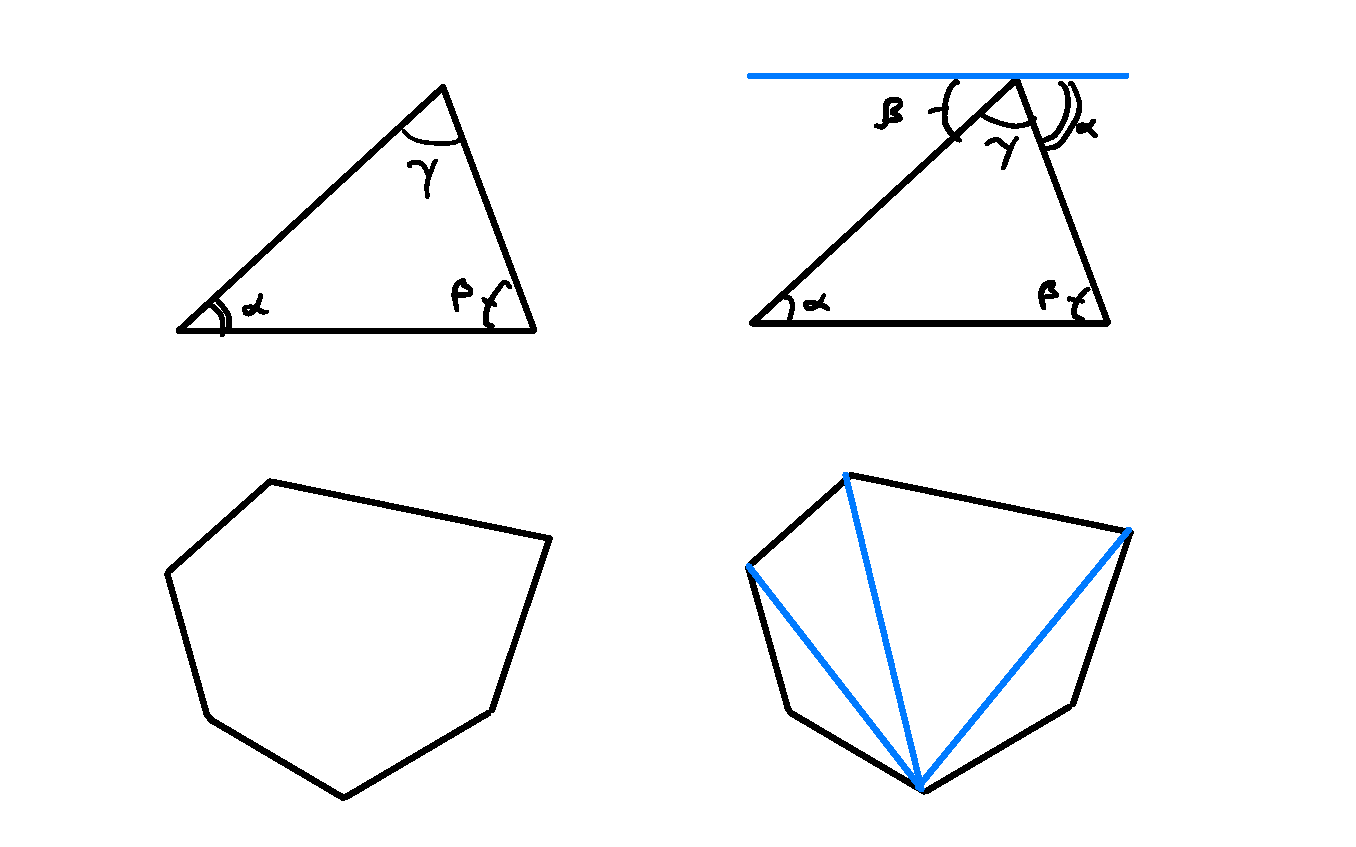
\includegraphics[width=.3\textwidth]{curvature/convex-angles}
\caption{Top row: the sum of  the interior angles of a triangle is $\pi$.
Bottom row: the sum of the interior angles of a convex polygon on $n$ edges is $(n-2)\pi$.}
\label{fig:angles}
\end{figure}


There are several ways to define curvature in the discrete setting \cite{Crane:2013},
this definition will be used in the poof of the discrete Gauss-Bonnet in \secref{proof}.

''For a discrete planar curve we can define the curvature at a vertex as the distance on the unit circle between the two adjacent normals'' \cite{Crane:2013}.

\begin{definition}[Discrete Gaussian curvature \cite{upadhyay2015}]\label{def:discrete-curvature-vertex}

The discrete \EMPH{Gaussian curvature} at a vertex $v$ is the area on the unit sphere bounded by a spherical polygon whose vertices are the unit normals of the faces around $v$.

\end{definition}


\begin{figure}[htb]
\centering
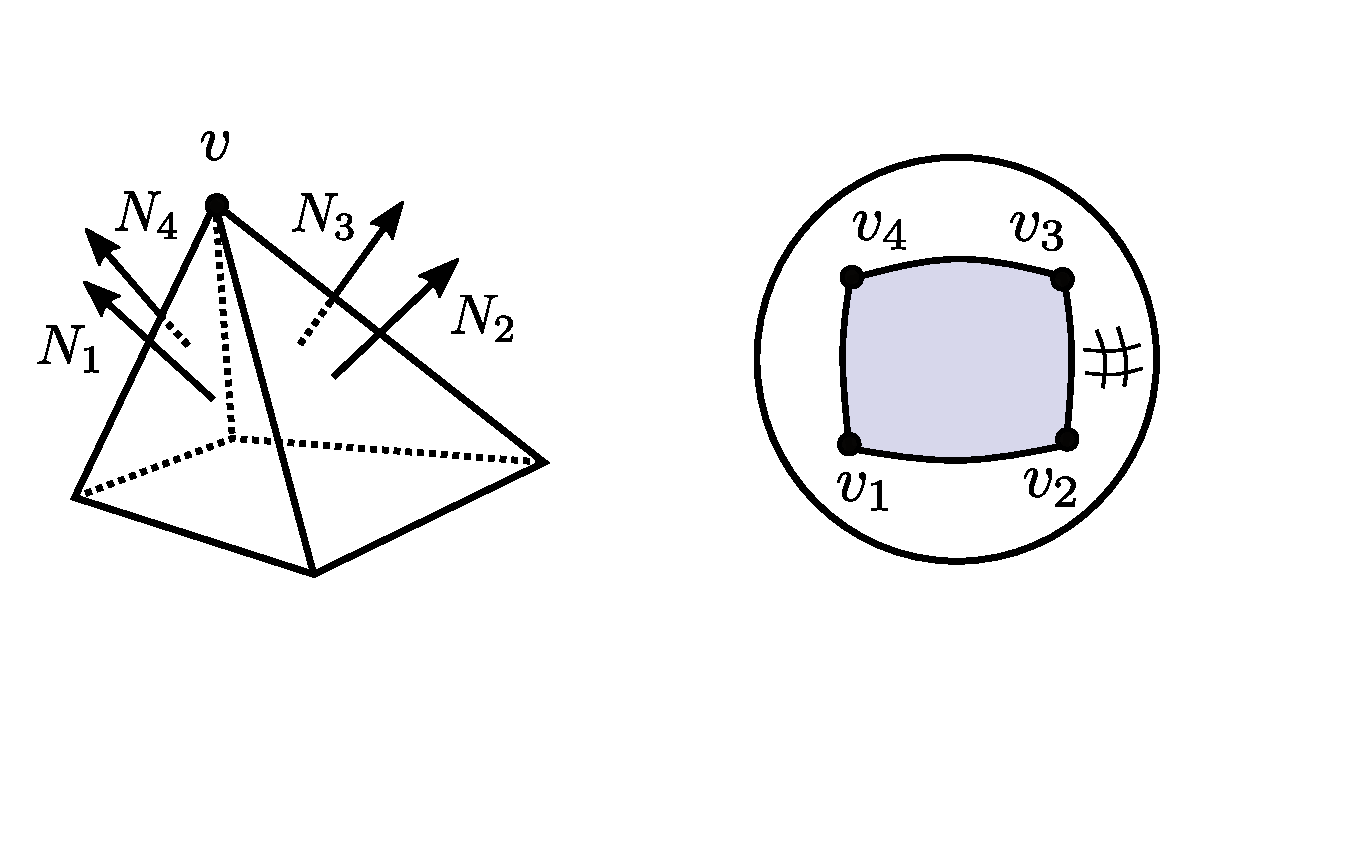
\includegraphics[width=.3\textwidth]{curvature/discrete-curvature}
\caption{The discrete curvature at vertex $v$ is the area drawn on the sphere.}
\label{fig:discrete-curvature}
\end{figure}

The \EMPH{angle defect} at a vertex $d(v)$ is the difference between $2\pi$ and
the sum of the incident angles.  Let $F_v$ denote the faces containing $v$  
and let $\alpha_f$  denote the interior  angle of face $f$ at $v$, then
$$d(v):=2\pi -\sum_{f\in F_v}\alpha_f.$$

The angle defect is equal to the discrete curvature in \defref{discrete-curvature-vertex}.

\subsection{The Euler Characteristic}

Properties of topological spaces that remain unchanged by homeomorphisms are called
\EMPH{topological invariants}. One such invariant is the Euler characteristic.
Originally defined for polyhedra, the \EMPH{Euler Characteristic} for surfaces $\chi$ is the 
the number of vertices minus the number of edges plus  the number of faces, $\chi=V-E+F.$
In higher dimensions, for a triangulated space $X$ the Euler characteristic is 
$\chi(X)=k_0-k_1+k_2-k_3+\ldots$ where $k_n$ is the number of simplices of dimension $n.$
A  graph  is \EMPH{planar} if it can be drawn in the plane with intersections only occuring
at vertices.
For a planar graphs $V-E+F=2$, Eppstein maintains a collection of proofs of this \cite{eppstein-proofs}.
We include the the following proof from Eppstein's list attributed to Thurston
 \cite{thurston}. For any planar graph we can map the graph on to the two sphere
 using stereographic projection.
 
\begin{theorem}[Euler Characteristic for Planar Graphs]\label{thm:euler}
For any planar graph on the 2-sphere we have $V-E+F=2.$
\end{theorem}

\begin{proof}
If needed, perturb the triangulation so that the north and south poles are 
inside of a two faces and there are no vertical edges. At each vertex place a unit positive
charge, at the center of each edge place a unit negative charge and put a unit positive
charge in the middle of each face. Slam the sphere on the ground so that all charges
on the edges and vertices are moved into the face below them. For faces that do not contain a pole
the net charge will be zero, the northern boundary consists of an alternating sequence
of edges and vertices  beginning  and ending with an edge.
The face containing the north pole has a unit positive charge, and the face containing the south
pole contains positive four units of charge and negative three units of charge.
Thus, the total charge is two.

\end{proof}

\section{The Gauss-Bonnet Theorem}



The Gauss-Bonnet theorem for regular surfaces states

\begin{theorem}[The Continuous Gauss-Bonnet Theorem] \label{thm:g-b-c}

If $M$ is a regular surface with boundary $\partial M$ then
	$$\int_{M} K dA+ \int_{\partial M} k_g ds + \sum_i \beta_i= 2\pi \chi(M)$$
	where  $K$ is Gaussian curvature,
	 $k_g$ is the geodesic curvature,
	 each $\beta_i$  is an exterior angle at a vertex of the boundary and
	$\chi$ is the Euler characteristic.
\end{theorem}


The  Gauss-Bonnet theorem is  telling us, if we add up curvature
at each vertex the sum will be $2\pi$ times to Euler characteristic.
The curvature at each vertex is computed by considering a 'local' neighborhood
around the vertex and we learn global topological information. Thus, the Gauss-Bonnet 
theorem is an example of a local to global principle. 
Conversely, if we know the Euler characteristic we can learn about the curvature
at individual points. We will often use the theorem to prove the existence of
a vertex with a desirable amount of curvature.



\subsection{Banchoff's Proof}
We now include a proof of a combinatorial version of the theorem due to Banchoff
\cite{banchoff_critical_1970}. We will first use another local to global theorem,
the Critical Point theorem, which we now define.
Given a regular surface embedded in $\R^3$ consider a line $\ell$ and define a linear height function $h:M \to \R$
to be the projection of all of $\R^3$ on to the line $\ell$. A point $p$ on $M$
is a \emph{critical point} for $\ell$ if the tangent plane at $p$ is perpendicular to $\ell$.
All points on $M$ that are not critical are \emph{ordinary point}.
Critical points can be classified into three categories, maxima, minima, and saddle points.
We define the \emph{index} of a critical point, denoted $i(p,h)$, to be 
$i(p,h)=1$ if $p$ is a  local maximum of minimum and $i(p,h)=-1$ is $p$ is a saddle point.
The \emph{Critical  Point theorem} states that if the number of critical points is finite
then 
$$\sum_{p\ \textrm{critical}} i(p,h)=\chi(M).$$



 \begin{figure}[htb]
         \centering
        \begin{subfigure}[b]{0.35\textwidth}
         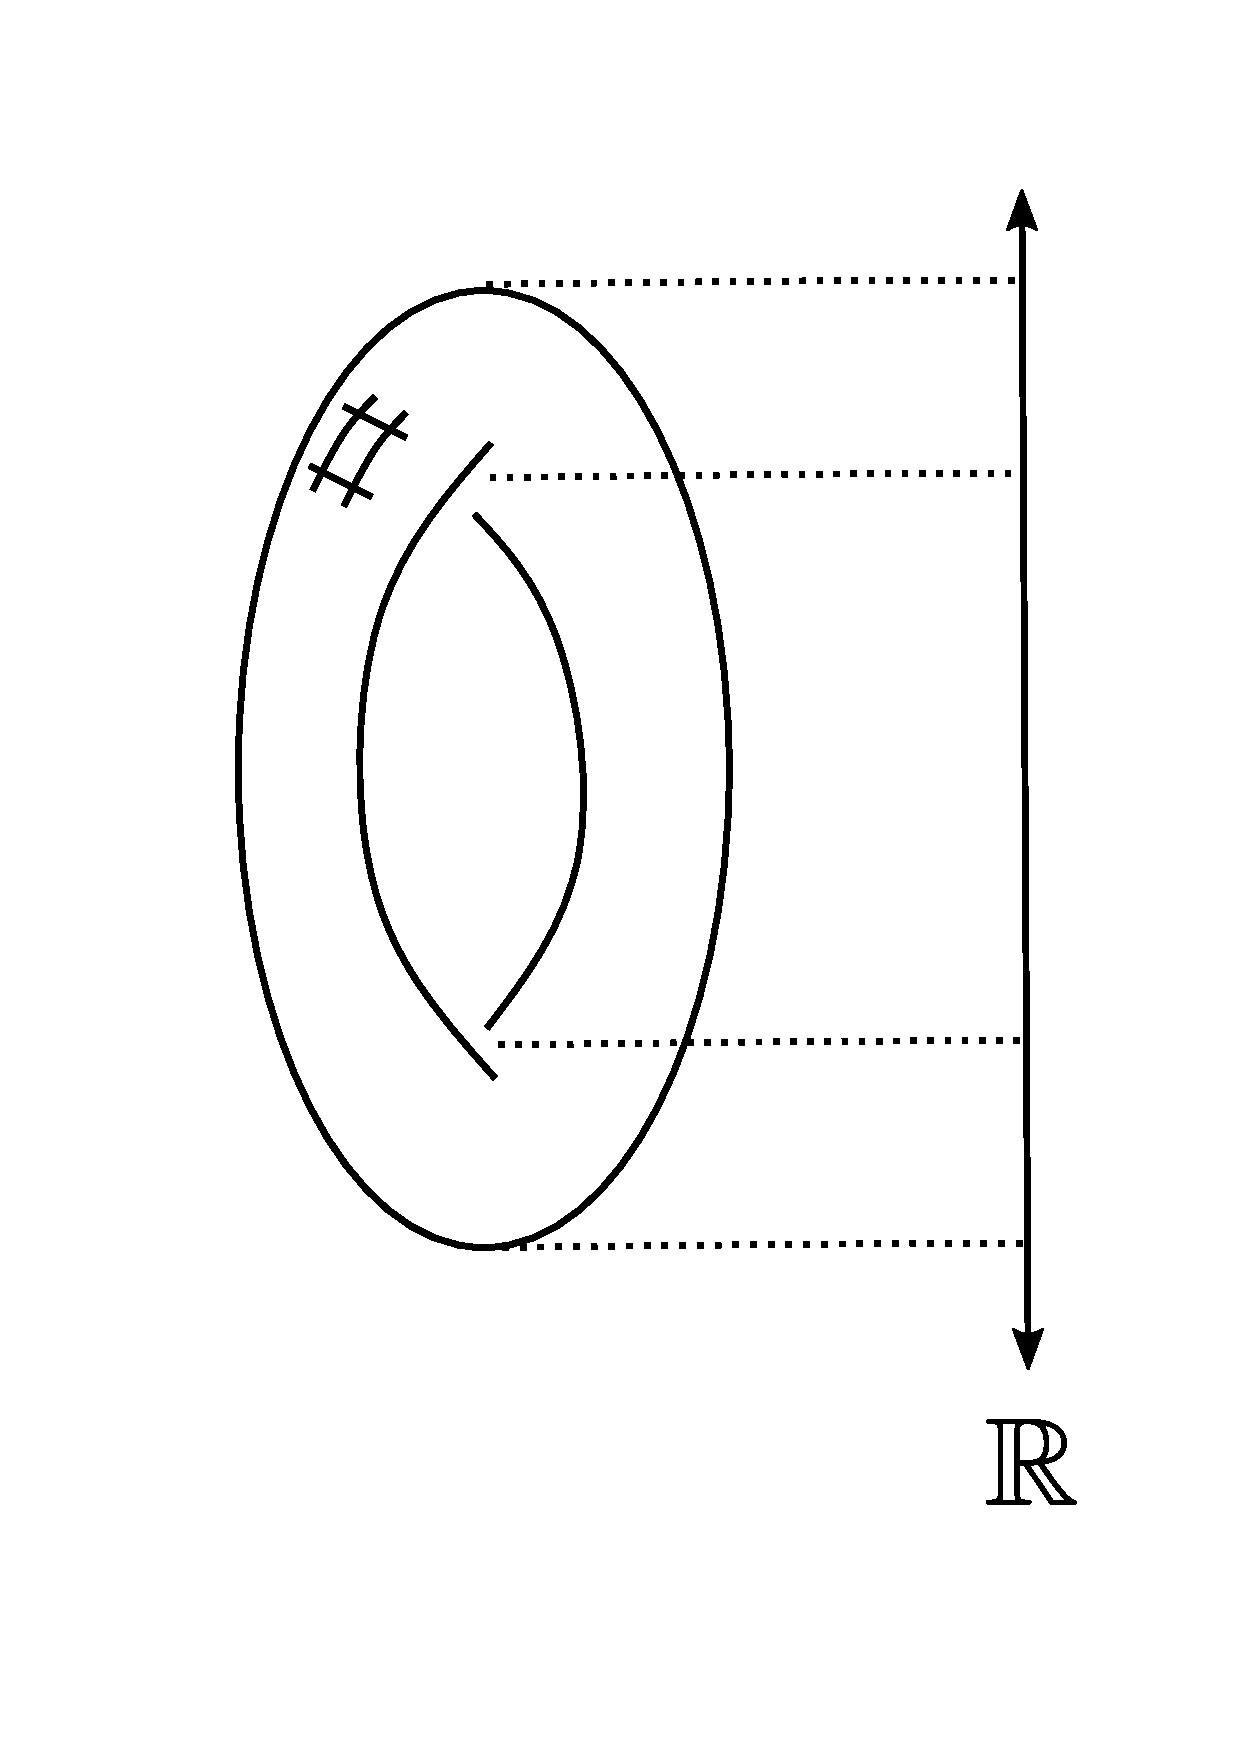
\includegraphics[width=\textwidth]{chapter-3/torus}
         \caption{Spherical triangle.}
 	 \label{fig:sphere-triangle}
       \end{subfigure}
         \hspace{1cm}
         \begin{subfigure}[b]{0.35\textwidth}
         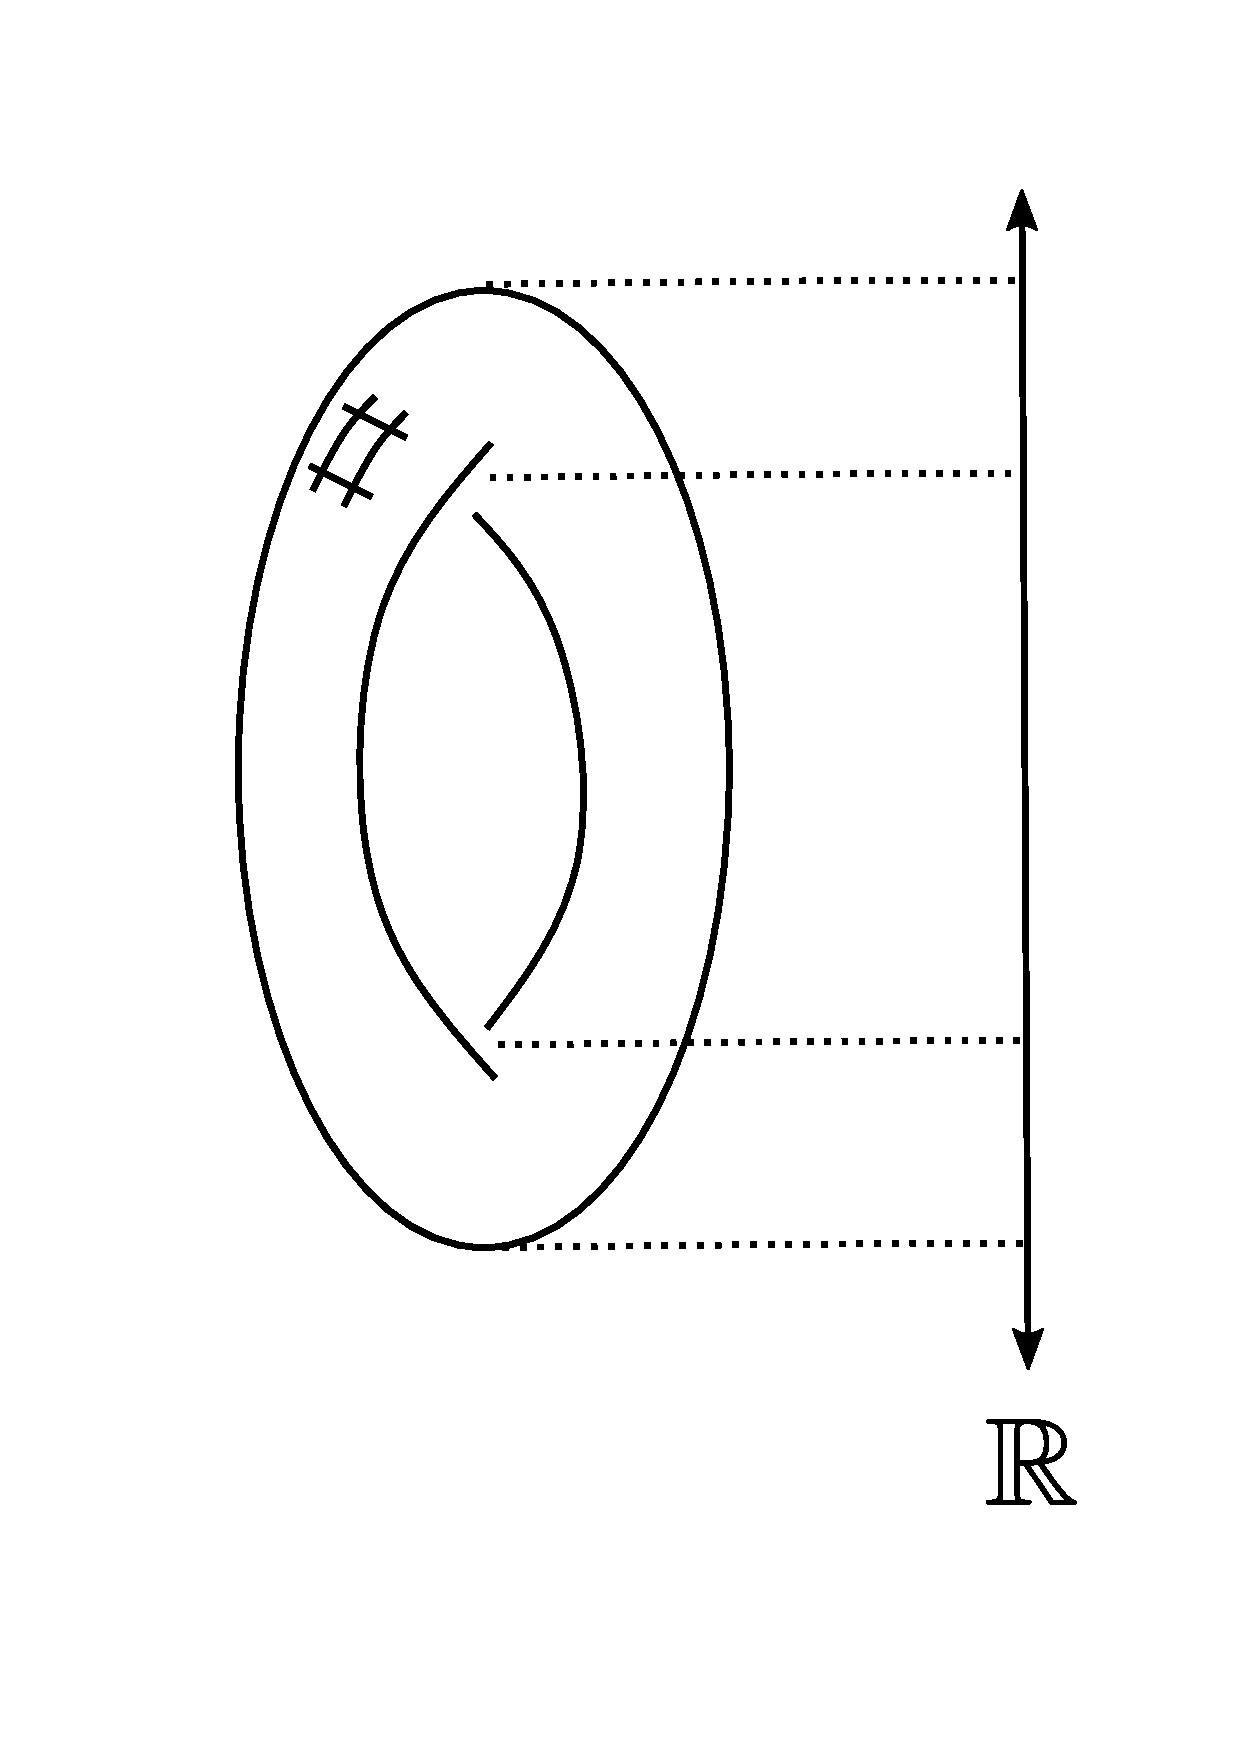
\includegraphics[width=\textwidth]{chapter-3/torus}
         \caption{A lune.}
          \label{fig:lune}
         \end{subfigure}
		\caption{(a) A triangle on the sphere.
 		(b) A lune with angle $\alpha$.
 		\label{fig:torus}}
 \end{figure}









\section{An Application to Computer Graphics}
\label{sec:graphics}

Computer graphics consist of meshes. Often, the mesh representing
an object contains more triangles than is necessary. One then wishes to
discard triangles without altering the geometry of the object \cite{simplify-mesh-1999}.


\cite{mmsb-2003}.











{
\small
\bibliographystyle{abbrv}
%\bibliographystyle{plainurl}
\bibliography{references}
}
\end{document}

